\subsection{Full-Wave Center-Taped Rectifier:}

Calculate the Voltage in $R_{L}$ ( $V_{0}$ ), the current in $R_{L}$ ( $I_{0}$ ), the Peak-Voltage ( $V_{p}$ ) at the output of the Transformer $V_{T}$ and $V_{p}$ - $V_{D}$:

\begin{figure}[H]
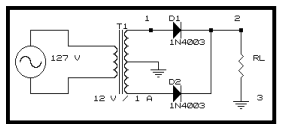
\includegraphics[scale=1]{fwct.png}
\centering \linebreak \linebreak Figure 5.4.0: Full-wave center-taped rectifier.
\end{figure}

{\bfseries\itshape Where:
\begin{tasks}
\task $R_{L}$ = 100 $\Omega$
\task $V_{D}$ = 0.7 V
\task $V_{T}$ = 12 V
\end{tasks}} \hfill

{\bfseries\itshape\color{Maroon}{Solution:}} \hfill \break

\begin{itemize}
\item {\bfseries\itshape\color{Violet}{For peak voltage at the transformer output:}} \hfill \break
{\bfseries\itshape\color{Brown}{
\begin{tasks}
\task Where: $V_{p}$ = $\frac{(\ \sqrt{2}\ )(\ V_{rms}\ )}{2}$.
\end{tasks}}}
\end{itemize}

\begin{ceqn}
\begin{align}
V_{p} = \frac{(\ \sqrt{2}\ )(\ V_{T}\ )}{2} = \frac{(\ \sqrt{2}\ )(\ 12 V\ )}{2} = 8.4 V.
\end{align}
\end{ceqn}

\begin{itemize}
\item {\bfseries\itshape\color{Violet}{For $V_{0}$:}} \hfill \break
{\bfseries\itshape\color{Brown}{
\begin{tasks}
\task Where: $V_{DC}$ = $(\ 2\ ) \frac{(\ \sqrt{2}\ )(\ V_{rms}\ )}{\ 2\ \pi}$.
\end{tasks}}}
\end{itemize}

\begin{ceqn}
\begin{align}
V_{0} = (\ 2\ )\frac{(\ \sqrt{2}\ )(\ V_{T}\ )}{\ 2\ \pi} = \frac{(\ 2\ )(\ \sqrt{2}\ )(\ 12 V\ )}{\ 2\ \pi} = 5.4 V.
\end{align}
\end{ceqn}

\begin{itemize}
\item {\bfseries\itshape\color{Violet}{For $I_{0}$:}} \hfill \break
{\bfseries\itshape\color{Brown}{
\begin{tasks}
\task Using Ohm's Law: $I$ = $\frac{V}{R}$.
\end{tasks}}}
\end{itemize}

\begin{ceqn}
\begin{align}
I_{0} = \frac{V_{0}}{R_{L}} = \frac{5.4V}{100\Omega} = 0.054 A.
\end{align}
\end{ceqn}

\begin{itemize}
\item {\bfseries\itshape\color{Violet}{Finally $V_{p}$ - $V_{D}$:}} \hfill \break
\end{itemize}

\begin{ceqn}
\begin{align}
V_{p} - V_{D} = 8.4 V - 0.7V = 7.7 V
\end{align}
\end{ceqn}

\pagebreak